\documentclass[12pt]{article}
\usepackage{amsmath,amssymb,bm,epsf,epsfig,graphicx,hyperref,physics, cleveref, subfig, slashed, stmaryrd, tensor, float}
\usepackage[backend=bibtex,natbib,style=numeric-comp,sorting=none, doi=false, isbn=false,url=false]{biblatex}
\addbibresource{ref}
\input epsf.sty
\topmargin -.5cm \textheight 21cm \oddsidemargin -.125cm
\textwidth 17cm
\setlength{\parskip}{0.7em}

\usepackage[]{todonotes}
\usepackage{tikz}
\usetikzlibrary{arrows.meta}

\usepackage[weather, alpine]{ifsym}

\definecolor{bisque}{rgb}{1.0, 0.89, 0.77}
\definecolor{forestgreen(web)}{rgb}{0.13, 0.55, 0.13}

\def\be{\begin{equation}}
\def\ee{\end{equation}}
\def\bea{\begin{eqnarray}}
\def\eea{\end{eqnarray}}
\def\ie{\begin{equation}\begin{aligned}}
\def\fe{\end{aligned}\end{equation}}
\numberwithin{equation}{section}
\def\mt{\bar}

\renewcommand{\title}[1]{\vbox{\center\LARGE{#1}}\vspace{5mm}}
\renewcommand{\author}[1]{\vbox{\center#1}\vspace{5mm}}
\newcommand{\address}[1]{\vbox{\center\em#1}}
\newcommand{\email}[1]{\vbox{\center\tt#1}\vspace{5mm}}

\newtheorem{theorem}{Theorem}
\newtheorem{proposition}{Proposition}
\newtheorem{lemma}{Lemma}
\newtheorem{definition}{Definition}

\begin{document}

\unitlength = .8mm

\begin{titlepage}

\begin{center}

\hfill \\
\hfill \\
\vskip 1cm

\title{Bosonic String Amplitudes From Ribbon Graphs}

\author{Sam Christian, Ben Mazel, Jaroslav Scheinpflug, Yuchen Wang, Xi Yin, Yutai Zhang}

\address{Jefferson Physical Laboratory, Harvard University,
Cambridge, MA 02138 USA
}

\email{yuchen\_wang@fas.harvard.edu, xiyin@fas.harvard.edu\\ (please enter your email by yourself)}

\end{center}

\abstract{We develop a new method for numerically computing higher-genus CFT correlators and string amplitudes based on Kontsevich's ribbon graph parametrization of the moduli space $\mathcal{M}_{g,n}$ of punctured Riemann surfaces. Using this method, we compute the compact boson partition functions as well as the moduli space integrand for bosonic string vacuum amplitudes at higher genus. Our results are checked against known analytic formulae, including T-duality of the compact boson and Mumford forms relevant to bosonic string amplitudes.}

\vfill

\end{titlepage}

\eject

\begingroup
\hypersetup{linkcolor=black}

\tableofcontents

\endgroup

\section{Introduction}


\section{Riemann surfaces from ribbon graphs}

\subsection{Kontsevich's isomorphism}

In this section, we review Kontsevich's parametrization of the moduli space $\mathcal{M}_{g,n}$ of genus-$g$, $n$-punctured Riemann surfaces by ribbon graphs \cite{Kontsevich:1992ti}. Specifically, $\mathcal{M}_{g,n}$ can be parametrized via the moduli space $\mathcal{M}_{g,n}^{\text{comb}}$ of metric ribbon graphs through Kontsevich's isomorphism 
\ie
\mathcal{M}_{g,n}\times \mathbb{R}_+^n \xrightarrow{\sim} \mathcal{M}_{g,n}^{\text{comb}}.
\fe
Here, each point of $\mathcal{M}_{g,n}^{\text{comb}}$ corresponds to a genus-$g$, $n$-faced metric ribbon graph, and the $n$ positive numbers in $\mathbb{R}_+^n$ parametrize the total edge length around each face.

This isomorphism can be explicitly constructed using the Strebel differential, defined as the unique quadratic differential $\omega = \varphi(z)dz^2$ given by the following theorem \cite{Strebel:1967, Strebel:1984}.
\begin{theorem}
Let $\Sigma$ be a genus-$g$ Riemann surface with $n$ punctures $\{z_1,\cdots, z_n\}$. Given a positive number $p_i\in \mathbb{R}_+$ for each puncture, if $n\geq 1$ and $2-2g-n<0$, there exists a unique quadratic differential $\omega = \varphi(z)dz^2$ that satisfies
\begin{enumerate}
\item $\omega$ is holomorphic on $\Sigma\backslash\{z_1,\cdots z_n\}$, and $\omega$ has a double pole at each $z_i$.
\item The union of all non-compact horizontal trajectories of $\omega$ has measure zero.
\item Each compact horizontal trajectory of $\omega$ is a simple loop around one of the punctures $z_i$. Horizontal trajectories $\gamma_i$ around puncture $z_i$ satisfy
\ie
\oint_{\gamma_i}\sqrt{\varphi(z)}\, dz =2\pi p_i.
\label{lengthconst}
\fe
\end{enumerate}
\end{theorem}

% All figures are temporary. We should redraw them in tikZ...
\begin{figure}
    \begin{center}
        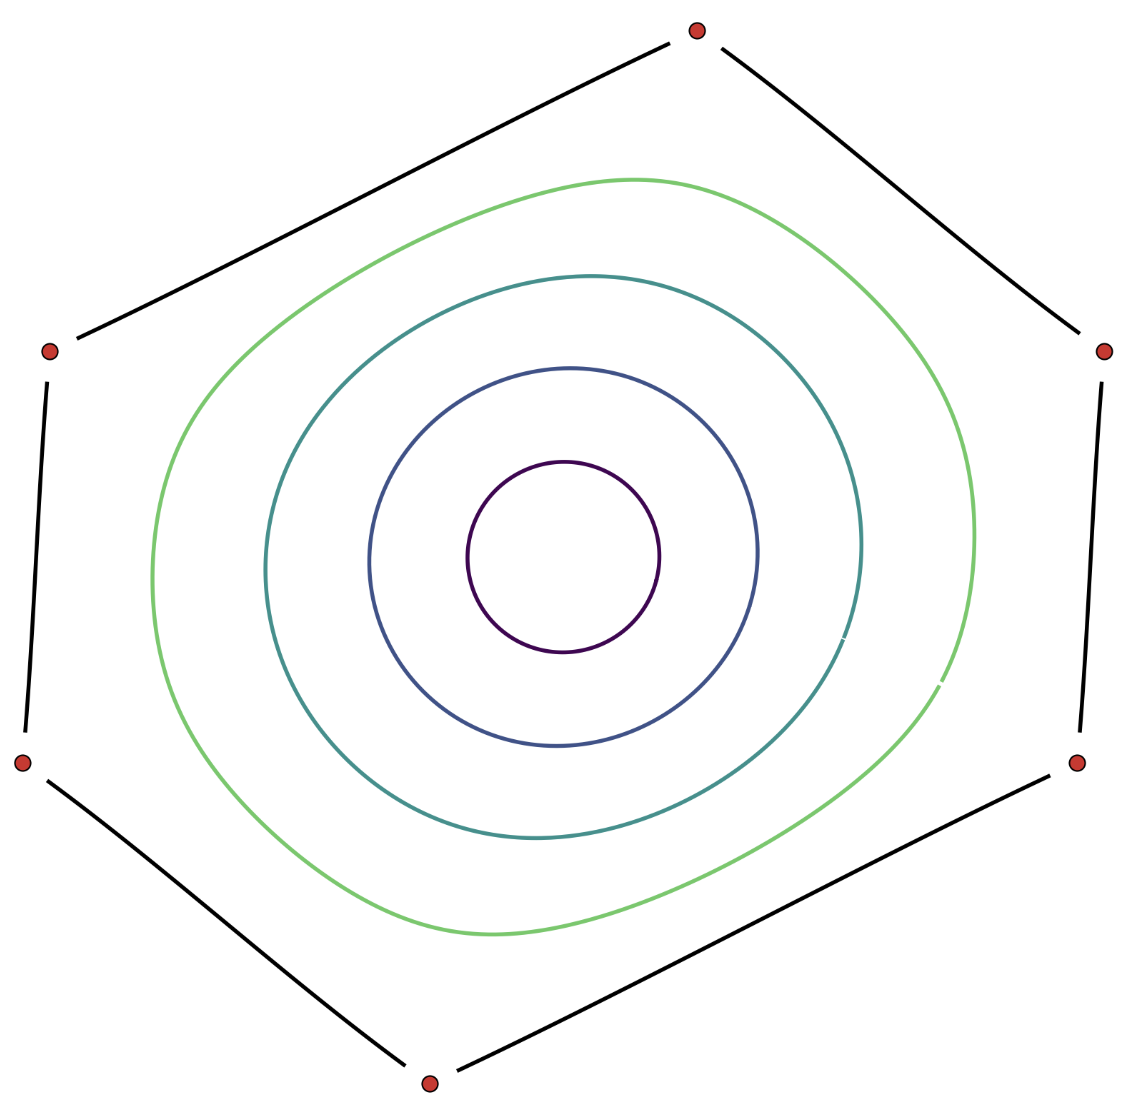
\includegraphics[scale=0.3]{figures/celldecompSigma.png}
    \end{center}
    \caption{Horizontal trajectories of the Strebel differential $\omega$. The red points correspond to the zeroes of $\omega$, the black lines are the non-compact horizontal trajectories, and the colored lines are the compact horizontal trajectories.}
    \label{celldecompSigma}
\end{figure}

It can be proved that each non-compact horizontal trajectory of $\omega$ is critical, namely that it is bounded by two zeroes of $\omega$. The union of all non-compact horizontal trajectories then forms a graph $\Gamma$ with $n$ faces, whose vertices are the zeroes of $\omega$ and whose edges are the non-compact horizontal trajectories. The Riemann surface $\Sigma$ can be divided into $n$ domains $D_i$, each swept out by the compact horizontal trajectories around $z_i$, as illustrated in figure \ref{celldecompSigma}. This gives a cell decomposition of $\Sigma$, in which the 2-cells are the domains $D_i$, while the 1-cells and 0-cells are the edges and vertices of the graph $\Gamma$, respectively. If we define the conformally flat metric
\ie ds^2=|\varphi(z)|dzd\bar{z},
\label{flatcylmetric}\fe
then the condition \eqref{lengthconst} tells us that all compact horizontal trajectories around $z_i$ have the same length $2\pi p_i$, and the domains $D_i$ have the geometry of a flat semi-infinite cylinder or equivalently a disk. On the domain $D_i$, one can define the disk coordinates $w_i$ to be
\ie
w_i(z) = \exp\left(\frac{i}{p_i}\int^z \sqrt{\omega}\right),
\label{diskcoord}
\fe
then the compact horizontal trajectories will have constant radius $|w_i|$, and the puncture $z_i$ will be located at $w_i=0$. The metric \eqref{flatcylmetric} will take the form
\ie
ds^2 = p_i^2 |w_i|^{-2} dw_i d\bar{w}_i.
\label{diskmetric}
\fe

The map $\mathcal{M}_{g,n}\times \mathbb{R}_+^n \rightarrow \mathcal{M}_{g,n}^{\text{comb}}$ is constructed as follows. Since the edge lengths and the cyclic order of edges at each vertex are preserved under biholomorphism, the graph $\Gamma$ comes with the structure of a metric ribbon graph. The map $\mathcal{M}_{g,n}\times \mathbb{R}_+^n \rightarrow \mathcal{M}_{g,n}^{\text{comb}}$ is then defined by sending $(\Sigma, \{p_i\})$ to the metric ribbon graph $\Gamma$ constructed in this way. From a metric ribbon graph $\Gamma$, the Riemann surface $\Sigma$ can be reconstructed by gluing a semi-infinite flat cylinder along each face of $\Gamma$, where the circumference of the cylinder is equal to the total edge length around that face, as shown in figure \ref{gluingcylinders}. This process defines the inverse map $\mathcal{M}_{g,n}^{\text{comb}}\rightarrow \mathcal{M}_{g,n}\times \mathbb{R}_+^n$.

\begin{figure}
    \begin{center}
        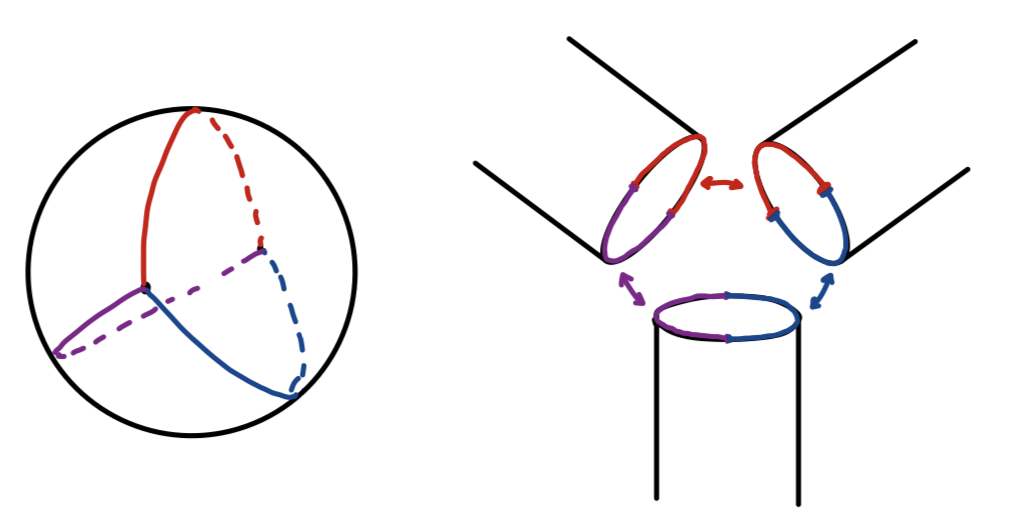
\includegraphics[scale=0.5]{figures/gluingcylinders.png}
    \end{center}
    \caption{Reconstructing a 3-punctured sphere by gluing 3 semi-infinite cylinders. The left picture shows the ribbon graph $\Gamma$.}
    \label{gluingcylinders}
\end{figure}

The combinatorial moduli space $\mathcal{M}_{g,n}^{\text{comb}}$ comes with a natural cell decomposition, in which each cell is labelled by the topology, or combinatorial type, of the ribbon graph. In particular, the top-dimensional cells correspond to trivalent graphs, namely graphs with only cubic vertices. In this case, each zero of the Strebel differential will be of degree 1. The full combinatorial moduli space $\mathcal{M}_{g,n}^{\text{comb}}$ is obtained by gluing these cells together along boundaries where one or more edge lengths degenerate to zero. For a trivalent graph with $n$ faces, its dual graph defines an $n$-vertex triangulation of the Riemann surface $\Sigma$, and the number of top-dimensional cells within $\mathcal{M}_{g,n}^{\text{comb}}$ can be counted by enumerating $n$-vertex triangulations on $\Sigma$. 

In the rest of this paper, we focus on the case of Riemann surfaces with a single puncture. In this case, the Riemann surface $\Sigma$ can be reconstructed from the ribbon graph by identifying segments on the boundary of a unit disk $D$, with the puncture located at the origin of $D$. The example of reconstructing a 1-punctured torus by gluing boundary segments of $D$ is illustrated in figure~\ref{gluingdisk}. 

\begin{figure}
    \begin{center}
        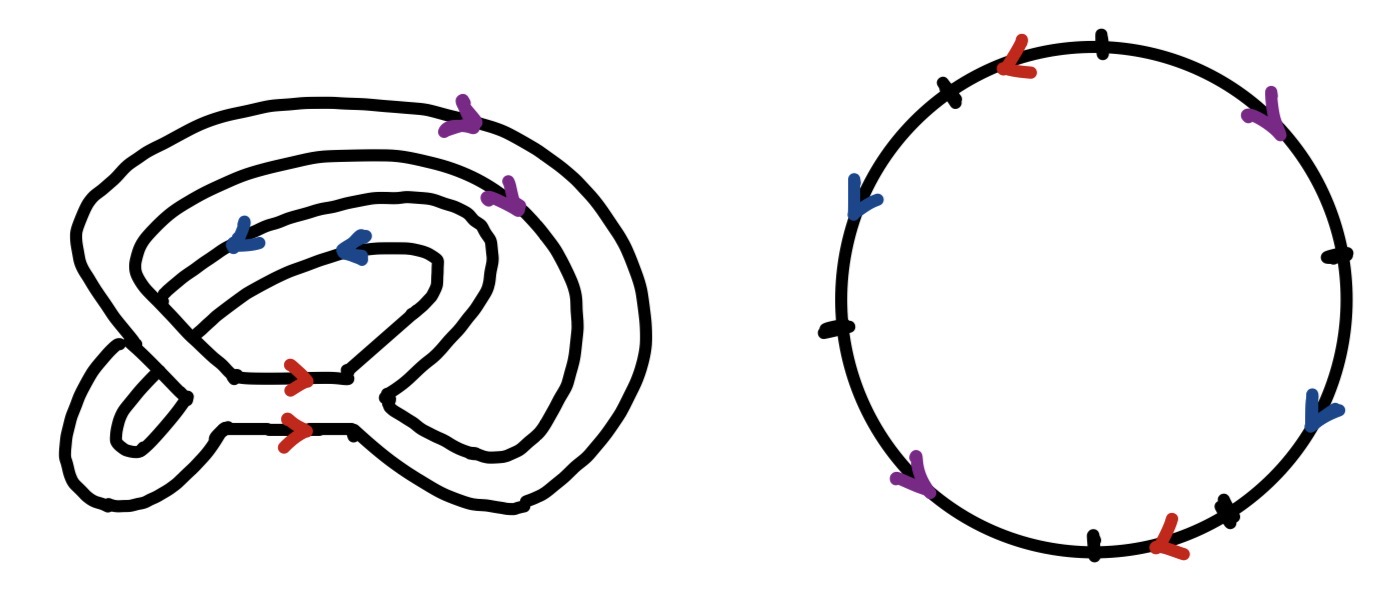
\includegraphics[scale=0.2]{figures/gluingdisk.jpg}
    \end{center}
    \caption{Reconstructing a 1-punctured torus by gluing boundary segments of the unit disk. Note that the boundary segments are glued in the opposite orientation.}
    \label{gluingdisk}
\end{figure}

Since the top-dimensional cells in $\mathcal{M}_{g,1}^{\text{comb}}$ correspond to trivalent graphs, the ribbon graph at a generic point in the moduli space has only cubic vertices. The number of vertices $V$ and edges $E$ in the ribbon graph $\Gamma$ therefore satisfy $3V=2E$. Together with Euler's formula $V-E+F=2-2g$, one can find
\ie E=6g-3,\quad V=4g-2.\fe 
Thus, reconstructing $\Sigma$ requires gluing $2E=6(2g-1)$ segments along the boundary of $D$, and different ways of gluing correspond to different topologies of the ribbon graph. The number of one-vertex triangulations of a genus-$g$ surface was determined by Bacher and Vdovina \cite{BACHER200213}, and the corresponding numbers of ribbon graph topologies are listed in table \ref{topologynumber}. 

\begin{table}
\begin{center}
\begin{tabular}{cccc}
\hline
Genus & Number of ribbon graph topologies \\ \hline
1     & 1                                 \\
2     & 9                                 \\
3     & 1726                              \\
4     & 1349005                           \\
5     & 2169056374                        \\ \hline
\end{tabular}
\end{center}
\caption{Number of topologies of genus-$g$ ribbon graphs with a single face.}
\label{topologynumber}
\end{table}

\subsection{Holomorphic data from ribbon graphs: Genus 1}

Given the metric ribbon graph $\Gamma$, one can numerically compute a basis of holomorphic 1-forms on $\Sigma$. For simplicity, we first present the algorithm for solving the holomorphic 1-form $f(z)dz$ on a genus-1 surface.

The 1-punctured torus can be reconstructed by gluing 3 pairs of boundary segments on the unit disk. For genus 1, there is only one ribbon-graph topology, and the corresponding gluing map is the same as the one illustrated in figure \ref{gluingdisk}. If we parametrize the unit circle by the angular coordinate $\sigma \in (0,2\pi)$, the gluing map reads
\ie
&\sigma \sim \pi + \theta_1 - \sigma, \quad 0<\sigma<\theta_1,\\
&\sigma \sim \pi + \theta_1 + \theta_2 - \sigma, \quad \theta_1 <\sigma<\theta_2,\\
&\sigma \sim 2\pi + \theta_2 - \sigma,\quad \theta_2 < \sigma < \pi.
\label{gluinggenus1}
\fe
The angles $\theta_{1}, \theta_2-\theta_1, \pi-\theta_2$ are the angular sizes of the three segments. In other words, they are the edge lengths of the ribbon graph if we take the radius $p$ to be $1$. The moduli space $\mathcal{M}_{1,1}$ can be parametrized by the two angles $\theta_1, \theta_2$.

Let us denote the disk coordinate by $z$, where the unit circle is given by $|z|=1$. The holomorphic 1-form $f(z)dz$ should be regular for $|z|<1$, and it should diverge at the Strebel vertices, namely the zeroes $z=\pm 1$, $\pm e^{i\theta_1}$, and $\pm e^{i\theta_2}$ of the Strebel differential $\omega = \varphi(z)dz^2$. In the flat torus coordinate $u$, where the holomorphic 1-form is given by $du$, the disk coordinate $z$ can be related to $u$ by equation \eqref{diskcoord}, which implies
\ie
f^{-1}(z) = \frac{du}{dz} = iz\sqrt{\varphi(u)}.
\fe
Since the ribbon graph $\Gamma$ has only cubic vertices, each zero $u_i$ of $\omega$ is of degree one, \textit{i.e.}, $\varphi(u)\sim (u-u_i)$ near $u_i$, and hence $f(z)$ will diverge like $(u-u_i)^{-1/2}$. Translating back to the disk coordinates, one can see the following divergent behavior of $f(z)$ around the zeroes $z_i$:
\ie
f(z) \sim (z-z_i)^{-1/3}.
\fe
Based on this divergent behavior, one can make the following ansatz:
\ie\label{fzoneform}
f(z) dz &= \frac{\sum_{n=1}^\infty a_n z^{n-1}}{(1-z^2)^{\frac13} (1-z^2 e^{-2 i \theta_1})^{\frac13} (1-z^2 e^{-2i \theta_2})^{\frac13}} dz.
\fe

The coefficients $a_n$ can be numerically determined as follows. We first discretize the unit circle into $L$ points where $L$ is an even number. The discretized points $z(k)$ are located at
\ie
z(k) = e^{\frac{2\pi i}{L}(k-\frac{1}{2})},\quad k=1,\cdots, L,
\fe
and we make the identifications
\ie
&z(k) \sim z(\tfrac{L}{2}+\ell_1+1-k),\quad 1\leq k \leq \ell_1,\\
&z(k) \sim z(\tfrac{L}{2}+2\ell_1+\ell_2+1-k),\quad \ell_1 \leq k \leq \ell_1+\ell_2,\\
&z(k) \sim z(L+\ell_1+\ell_2+1-k),\quad \ell_1+\ell_2\leq k \leq \tfrac{L}{2},\\
\fe
as a discretized version of the gluing map \eqref{gluinggenus1}. We will denote the point identified with $z(k)$ by $z(k')$. The relative segment lengths $\tfrac{\ell_1}{L}, \tfrac{\ell_2}{L}$ can be identified with the moduli $\theta_1, \theta_2-\theta_1$, respectively. The Strebel vertices $\pm 1,\pm e^{i\theta_1}, \pm e^{i\theta_2}$ are located halfway between the discretized points at the edges of identified sections of the boundary.

In order to solve \eqref{fzoneform}, we can truncate the Fourier coefficients $a_n$ by restricting to the lowest $\tfrac{L}{2}$ modes, normalize with $a_1=1$, and solve for $a_2,\cdots a_{L/2}$ by imposing the condition that $f(z)dz$ matches across identified discretized points:
\ie
{}&\frac{\sum_{n=1}^{L \over 2} a_n e^{in (2 \pi \frac{k-\frac 12}{L})} }{(1-e^{4i\pi \frac{k-\frac12}{L}})^{\frac13} (1- e^{4i \pi \frac{k-\frac12-\ell_1}{L} })^{\frac13} (1- e^{4i\pi \frac{k-\frac12-\ell_1 -\ell_2}{L} })^{\frac13}}\\
&\qquad\qquad = - \frac{\sum_{n=1}^{L \over 2} a_n e^{in (2 \pi \frac{k'-\frac 12}{L})} }{(1-e^{4i\pi \frac{k'-\frac12}{L}})^{\frac13} (1- e^{4i \pi \frac{k'-\frac12-\ell_1}{L} })^{\frac13} (1- e^{4i\pi \frac{k'-\frac12-\ell_1 -\ell_2}{L} })^{\frac13}}, ~~~~1 \leq k \leq \tfrac{L}{2},
\fe
where the relative sign is due to flipping the orientation of $dz$. 

\begin{figure}
    \begin{center}
        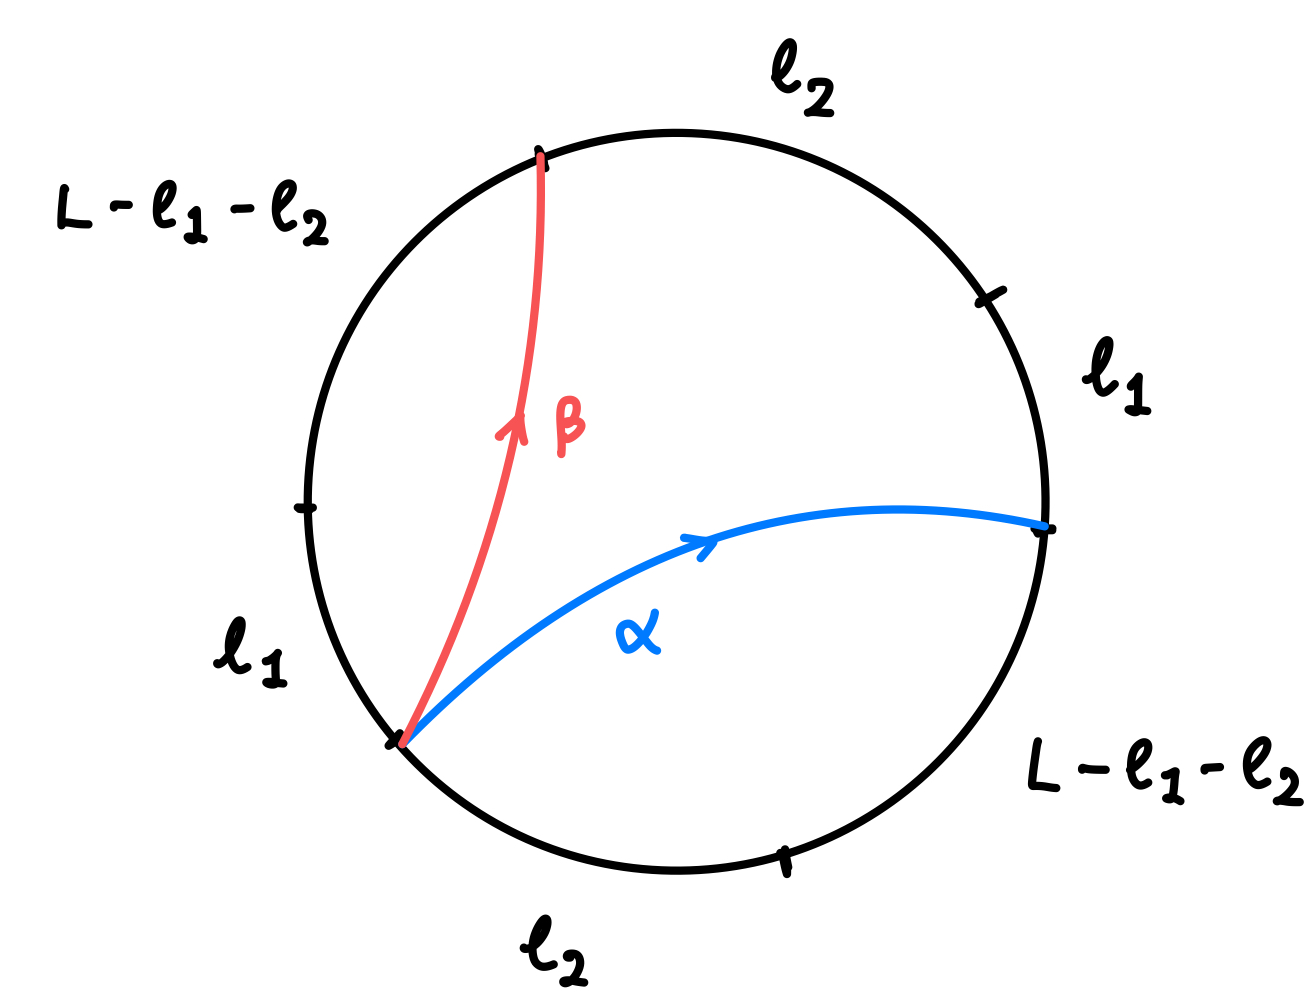
\includegraphics[scale=0.16]{figures/torus1cycles.jpeg}
    \end{center}
    \caption{Symplectic basis of 1-cycles on the torus.}
    \label{torus1cycles}
\end{figure}

Once the holomorphic 1-form is solved, we can numerically compute the usual complex modulus $\tau$ of the torus by integrating it against a symplectic basis $\alpha, \beta$ of 1-cycles
\ie
\tau = \frac{\int_\beta f(z)dz}{\int_\alpha f(z)dz}.
\fe
In the disk frame, both of these cycles are given by chords that connect the identified points, as illustrated in figure \ref{torus1cycles}.

\subsection{Holomorphic data from ribbon graphs: Higher genus}

The algorithm above can be generalized to the case of $g\geq 2$. The genus-$g$ Riemann surface can be reconstructed by gluing $12g-6$ boundary segments on the disk. Upon discretizing the unit circle into $L$ sites, the moduli space $\mathcal{M}_{g,1}$ can be parametrized by the $6g-4$ independent edge lengths.

Going counterclockwise from $z=1$, we label the boundary segments $S_i$ from $i=1$ to $i=12g-6$. The edges can be labelled by $E_a$ with $a=1,\cdots, 6g-3$, where each edge $E_a$ pairs two segments $S_{i_1(a)}$ and $S_{i_2(a)}$ and glues them with opposite orientation. The number of discretized sites contained in $E_a$ is denoted by $\ell_a$. We will always take $i_1(a)<i_2(a)$. Conversely, we denote the edge associated with segment $i$ by $a(i)$. The map $a(i)$ depends on the ribbon-graph topology. Given a ribbon-graph topology, the top-dimensional cells in $\mathcal{M}_{g,1}^{\text{comb}}$ can be parametrized by the relative edge lengths $\tfrac{\ell_a}{L}$. Using this language, the gluing map on the unit circle can be written as
\ie
z(k)\sim z\left(\sum_{j\leq i_1(a)}\ell_{a(j)}+\sum_{k< i_2(a)}\ell_{a(k)}-k+1\right),\quad \sum_{j<i_1(a)}\ell_{a(j)}+1\leq k \leq \sum_{j\leq i_1(a)}\ell_{a(j)},
\fe
and the Strebel vertices are located at
\ie
z_i = \exp\left(\frac{2\pi i}{L}\sum_{j<i}\ell_{a(j)}\right).
\fe
One additional complication is that, for higher genus, the independent boundary points are not simply $z(k)$ with $1\leq k \leq L/2+1$, since the segments in the same half-circle can be glued together. We denote the set of independent variables by $\mathcal{K}=\cup_{a=1}^{6g-3}\{k, k\in S_{i_1(a)}\}$.

On a genus-$g$ surface, there are $g$ linearly independent holomorphic 1-forms. We start with the following ansatz for each holomorphic 1-form
\ie
f(z)dz= \frac{\sum_{n=1}^\infty a_n z^{n-1}}{\prod_{i=1}^{12g-6}\left(1-z\exp\left({-\frac{2\pi i}{L}\sum_{j<i}\ell_{a(j)}}\right)\right)^{\frac{1}{3}}}dz,
\fe
and again solve for the coefficients $a_1,\cdots, a_{L/2}$ by matching the values of $f(z)dz$ on the identified boundary points. The resulting linear system of the coefficients $a_n$ will have a $g$-dimensional kernel. One can take the first $g$ coefficients of the $i$-th holomorphic 1-form $\omega_i=f^{(i)}(z)dz$ to be $a^{(i)}_n = \delta_{i,n}~(n=1,\cdots,g)$, and solve for the remaining $a^{(i)}_{g+1},\cdots, a^{(i)}_{L/2}$.

One can then pick a symplectic basis $\{\alpha_i, \beta_j\}$ of 1-cycles among all chords that connects identified Strebel vertices, whose intersection numbers satisfying
\ie
\alpha_i\cdot \alpha_j = \beta_i\cdot \beta_j = 0,\quad \alpha_i\cdot \beta_j = \delta_{ij},
\fe
and the period matrix $\Omega$ of the Riemann surface can be then be computed by
\ie
\Omega_{ij}=\mathcal{B}_{ik}(\mathcal{A}^{-1})_{kj},\quad \mathcal{A}_{ij}=\oint_{\alpha_i}\omega_j,\quad \mathcal{B}_{ij}=\oint_{\beta_i} \omega_j.
\fe
Further geometric quantities on the Riemann surface, such as the Riemann constant vector and the prime form, can be computed using the holomorphic 1-form and the period matrix. These quantities are used in the computation of $bc$ ghost correlators, and the details are presented in section \ref{somewhere}.

\section{Free boson CFT from ribbon graphs}

\section{Weyl anomaly and $bc$ ghosts}

\section{Compact boson at higher genus}

\section{Moduli space integrand of vacuum amplitudes}


\printbibliography
\end{document}
